\documentclass[11pt,letterpaper]{article}

\usepackage[margin=1in]{geometry}
\usepackage{graphicx}
\usepackage{booktabs}
\usepackage{caption}
\usepackage{subcaption}
\usepackage{hyperref}
\usepackage{xcolor}
\usepackage{titlesec}
\usepackage{enumitem}
\usepackage{microtype}
\usepackage{lmodern}
\usepackage[T1]{fontenc}

\hypersetup{
  colorlinks=true,
  linkcolor=black,
  urlcolor=teal,
  citecolor=teal,
}

\definecolor{teal-accent}{HTML}{20808D}
\definecolor{terra-accent}{HTML}{A84B2F}

\titleformat{\section}{\Large\bfseries\color{teal-accent}}{\thesection}{0.6em}{}
\titleformat{\subsection}{\large\bfseries}{\thesubsection}{0.6em}{}

\setlength{\parskip}{6pt}
\setlength{\parindent}{0pt}

\title{\textbf{Measuring Inequality After Taxes and Transfers:\\
\large A Reproducible Distributional Panel for the United States, 1979--2022}}
\author{Patrick Poleshuk\\
\small Independent pre-doctoral research project\\
\small Source code and data:
\href{https://github.com/Patrickkp1/tax-transfer-inequality}{\small github.com/Patrickkp1/tax-transfer-inequality}}
\date{May 2026}

\begin{document}

\maketitle

\begin{abstract}
\noindent The U.S.\ Census Bureau's official income measure, used in nearly all
public discussion of inequality, was designed in 1947 around an economy in which
roughly 90\% of household compensation arrived as cash. That economy no longer
exists: by 2017 about two-thirds of federal transfer payments to households
were non-cash (Medicare, Medicaid, SNAP, housing assistance, the EITC, the
refundable Child Tax Credit), and the federal tax code had become much more
progressive than it was in the early postwar period. Census's pretax,
cash-only construct counts neither side of the fiscal system, and the gap
between that measure and a complete income concept has grown substantially over
time. This paper builds a reproducible distributional accounting panel covering
all five income quintiles plus eight upper-tail groups (81--90, 91--95, 96--99,
Top 1, Top 0.1, Top 0.01, Top 0.001\%, and the Forbes 400) for tax years
1979--2022, supplementing Current Population Survey (CPS) microdata with
control totals from the Congressional Budget Office, Internal Revenue Service,
Office of Management and Budget, Bureau of Economic Analysis, Bureau of Labor
Statistics, Social Security Administration, and Giving USA. Once taxes and
transfers are accounted for, the top-to-bottom quintile income ratio in 2022
is 4.4\(\times\), not the 96\(\times\) gap implied by earned income alone, and
real after-tax-and-transfer income has risen for every quintile of the U.S.
distribution since 1979.
\end{abstract}

% =============================================================================
\section{Motivation}
% =============================================================================

In \emph{The Myth of American Inequality} (2022), Phil Gramm, Robert Ekelund, and
John Early argue that the standard Census Bureau measure of household income
provides a distorted picture of the U.S.\ income distribution because it
omits two large categories of income flows. First, the Census measure counts
only cash transfers as income; it excludes Medicare, Medicaid, SNAP, housing
assistance, and the refundable portions of the EITC and Child Tax Credit ---
in 1947 these represented less than 10\% of all transfers, but by 2017 they
were roughly two-thirds.\footnote{Gramm, Ekelund, and Early, \emph{The Myth of
American Inequality} (Rowman \& Littlefield, 2022), pp.\ 13--15.} Second, the
Census measure is a pretax measure: it ranks households by income before
federal, state, and local taxes are deducted, even though households at the
top of the distribution lose about 33\% of pretax income to taxes and households
at the bottom lose about 7\%. Both omissions push the official inequality measure
upward, and both have grown over time.

This project replicates Gramm et al.'s data architecture end-to-end from
public sources, with two main motivations:

\begin{enumerate}[leftmargin=*]
  \item To produce a fully reproducible panel that any researcher can rebuild
        from the original administrative documents, with every assumption
        traceable to a specific data file or peer-reviewed citation. The
        seven-stage pipeline described below ingests CPS microdata, eleven
        CBO supplemental tables, IRS Statistics of Income files, OMB
        Historical Tables, BEA NIPA tables, BLS expenditure surveys, and SSA
        trust fund data.
  \item To examine how the gap between Census's measure and a complete
        post-fiscal measure has evolved over a long horizon (1979--2022), and
        what that gap implies for the standard narrative about rising
        inequality.
\end{enumerate}

\section{Conceptual framework}

The income concept we attempt to measure for each household is

\begin{equation}
\text{IAT} \;=\; E + G + P - T
\end{equation}

\noindent (where IAT denotes ``income after taxes and transfers''),

\noindent where $E$ is earned income (wages plus employer benefits plus business and
financial income), $G$ is government transfers (the cash and non-cash sum), $P$
is private transfers (charitable transfers from households and institutions to
households), and $T$ is the household's total federal, state, and local tax
burden. This is the conventional ``post-fisc'' concept used in the CBO's
distributional analyses; we extend the CBO framework backward to 1979 and
forward to 2022, and we add private transfers as a fourth component.

The Census ``money income'' measure used in headline inequality statistics
is conceptually $E + G_{\text{cash}}$ --- it omits in-kind transfers
($G - G_{\text{cash}}$), all of $P$, and all of $T$. Households are also
ranked by money income, not by a post-fisc concept, so a low-income retiree
receiving \$30k in Medicare benefits and a working-age household earning
\$30k from wages appear in the same Census quintile despite having very
different consumption capacity.

\section{Data and method}

The pipeline produces five panel CSVs in five sequential stages, plus a final
ultra-top stage that reconciles the quintile-level panels with administrative
data on the very wealthy. All scripts are written in Python and are designed
to be self-contained and re-runnable from the underlying administrative files.

\subsection{Stage 1: Earned income}

CPS ASEC microdata (IPUMS, survey years 1980--2023) provides household-level
wages, business income, farm income, dividends, interest, rent, and
retirement income. Households are ranked by earned income within each survey
year using ASEC household weights. Employer-paid benefits (health insurance,
retirement contributions) are imputed using year-specific BLS Employer Costs
for Employee Compensation (ECEC) ratios applied to wages and salaries. A
constant adjustment of \$1{,}800 is added to bottom-quintile wages to capture
in-kind compensation not captured in the CPS, following Meyer and Sullivan
(2012).

\subsection{Stage 2: Government transfers}

National program totals come from administrative sources rather than from
self-reported CPS receipts (which substantially underreport in-kind
benefits): SSA Trustees Reports for OASI and SSDI; CMS National Health
Expenditure tables for Medicare (\emph{net of} beneficiary-paid Part B/D
premiums and out-of-pocket cost-sharing); BEA NIPA Table 3.12 for Medicaid,
SNAP, and other federal cash and in-kind transfers; OMB Historical Tables for
housing assistance; USDA Food and Nutrition Service tables for the National
School Lunch Program and WIC. Quintile distribution weights are taken from
CBO supplemental Tables 5 and 6, except for OASI receipts, which are
re-ranked by earned income from the CPS extract when available.

\subsection{Stage 3: Tax distribution}

Federal taxes --- personal income, payroll (OASDI plus Medicare HI), excise,
estate and gift, customs, FUTA, railroad retirement, and other retirement ---
come from CBO Tables 7 and 12 (per-household averages and quintile shares),
supplemented with OMB Historical Tables 2.1, 2.4, and 2.5 to break out
specific receipt categories. Corporate income tax is excluded from the
household burden, since households do not pay it directly.

State and local taxes are distributed from Tax Policy Center / Census State
\& Local Government Finance national totals using three keys: BLS Consumer
Expenditure Survey shares (sales and motor-vehicle taxes), CPS homeownership
times household income (property taxes), and CPS wage income (state income
taxes). The S\&L methodology uses year-specific BLS shares back to 1984 and
proxy weights for 1979--1983.

\subsection{Stage 4: Private transfers and assembly}

The Stage 4 script joins the three upstream panels and adds a private-transfer
component built from three independent data sources:

\begin{itemize}[leftmargin=*]
  \item \textbf{Component A: Child support and alimony.} CPS variables
        \texttt{INCCHILD}, \texttt{INCALIM}, and \texttt{INCALOTH}, distributed
        across quintiles using the Census Child Support Supplement (2018).
  \item \textbf{Component B: Informal cash assistance.} CPS variables
        \texttt{INCASIST} and \texttt{INCOTHER}, distributed using the
        normalized bivariate odds ratios from Karen (2023, LIS Working Paper
        No.~851, Table 2, Model 1).
  \item \textbf{Component C: Charitable giving received by households.} The
        Giving USA recipient series (1979--2022) is ingested from a CSV with
        ten recipient categories. Each category is multiplied by a
        household-directed fraction representing the share of donations that
        flow through to households as a transfer (Religion 5\%, Education
        5\%, Human Services 50\%, Foundations 0\%, Health 8\%,
        Public-Society Benefit 5\%, International Affairs 25\%, Arts and
        Environment 0\%, Individuals 100\%). The Giving USA CSV is verified
        against the \emph{Giving USA 2014 Data Tables} for 1979--2013 and
        against each subsequent annual highlights publication for 2014--2022.
\end{itemize}

\subsection{Stage 5: Ultra-top groups}

The CBO supplemental tables provide top-quintile sub-groups (81--90, 91--95,
96--99, and Top 1\%). To go above the Top 1\%, the script ingests IRS
Statistics of Income Table 4.1 Time Series (covers 2001--2022 for the Top
0.1\%, 0.01\%, and 0.001\%) and IRS Top 400 publications (1992--2014, with
T41TS-based extrapolations for 2015--2022). IRS Table 3 / 4.3 income-composition
files (\texttt{*in03etr*.xls} for 2014--2018, \texttt{*in43ts*.xls} for 2019--2022)
provide labor / capital / pass-through splits at the top of the distribution.

% =============================================================================
\section{Findings}
% =============================================================================

\subsection{The pretax-vs-postfisc gap}

Figure~\ref{fig:ratio} plots the top-to-bottom quintile ratio for the two
income concepts on a common log scale. The earned-income ratio rises from
24$\times$ in 1979 to 96$\times$ in 2022 --- a fourfold increase that is the
basis for most contemporary descriptions of rising inequality. After taxes
and transfers, the ratio rises from 2.3$\times$ to 4.4$\times$ --- still
upward-trending, but at a much smaller absolute level and at a substantially
lower rate of growth. The vertical distance between the two lines is the
amount of inequality the standard Census measure misses by ignoring the
fiscal system.

\begin{figure}[!htb]
\centering
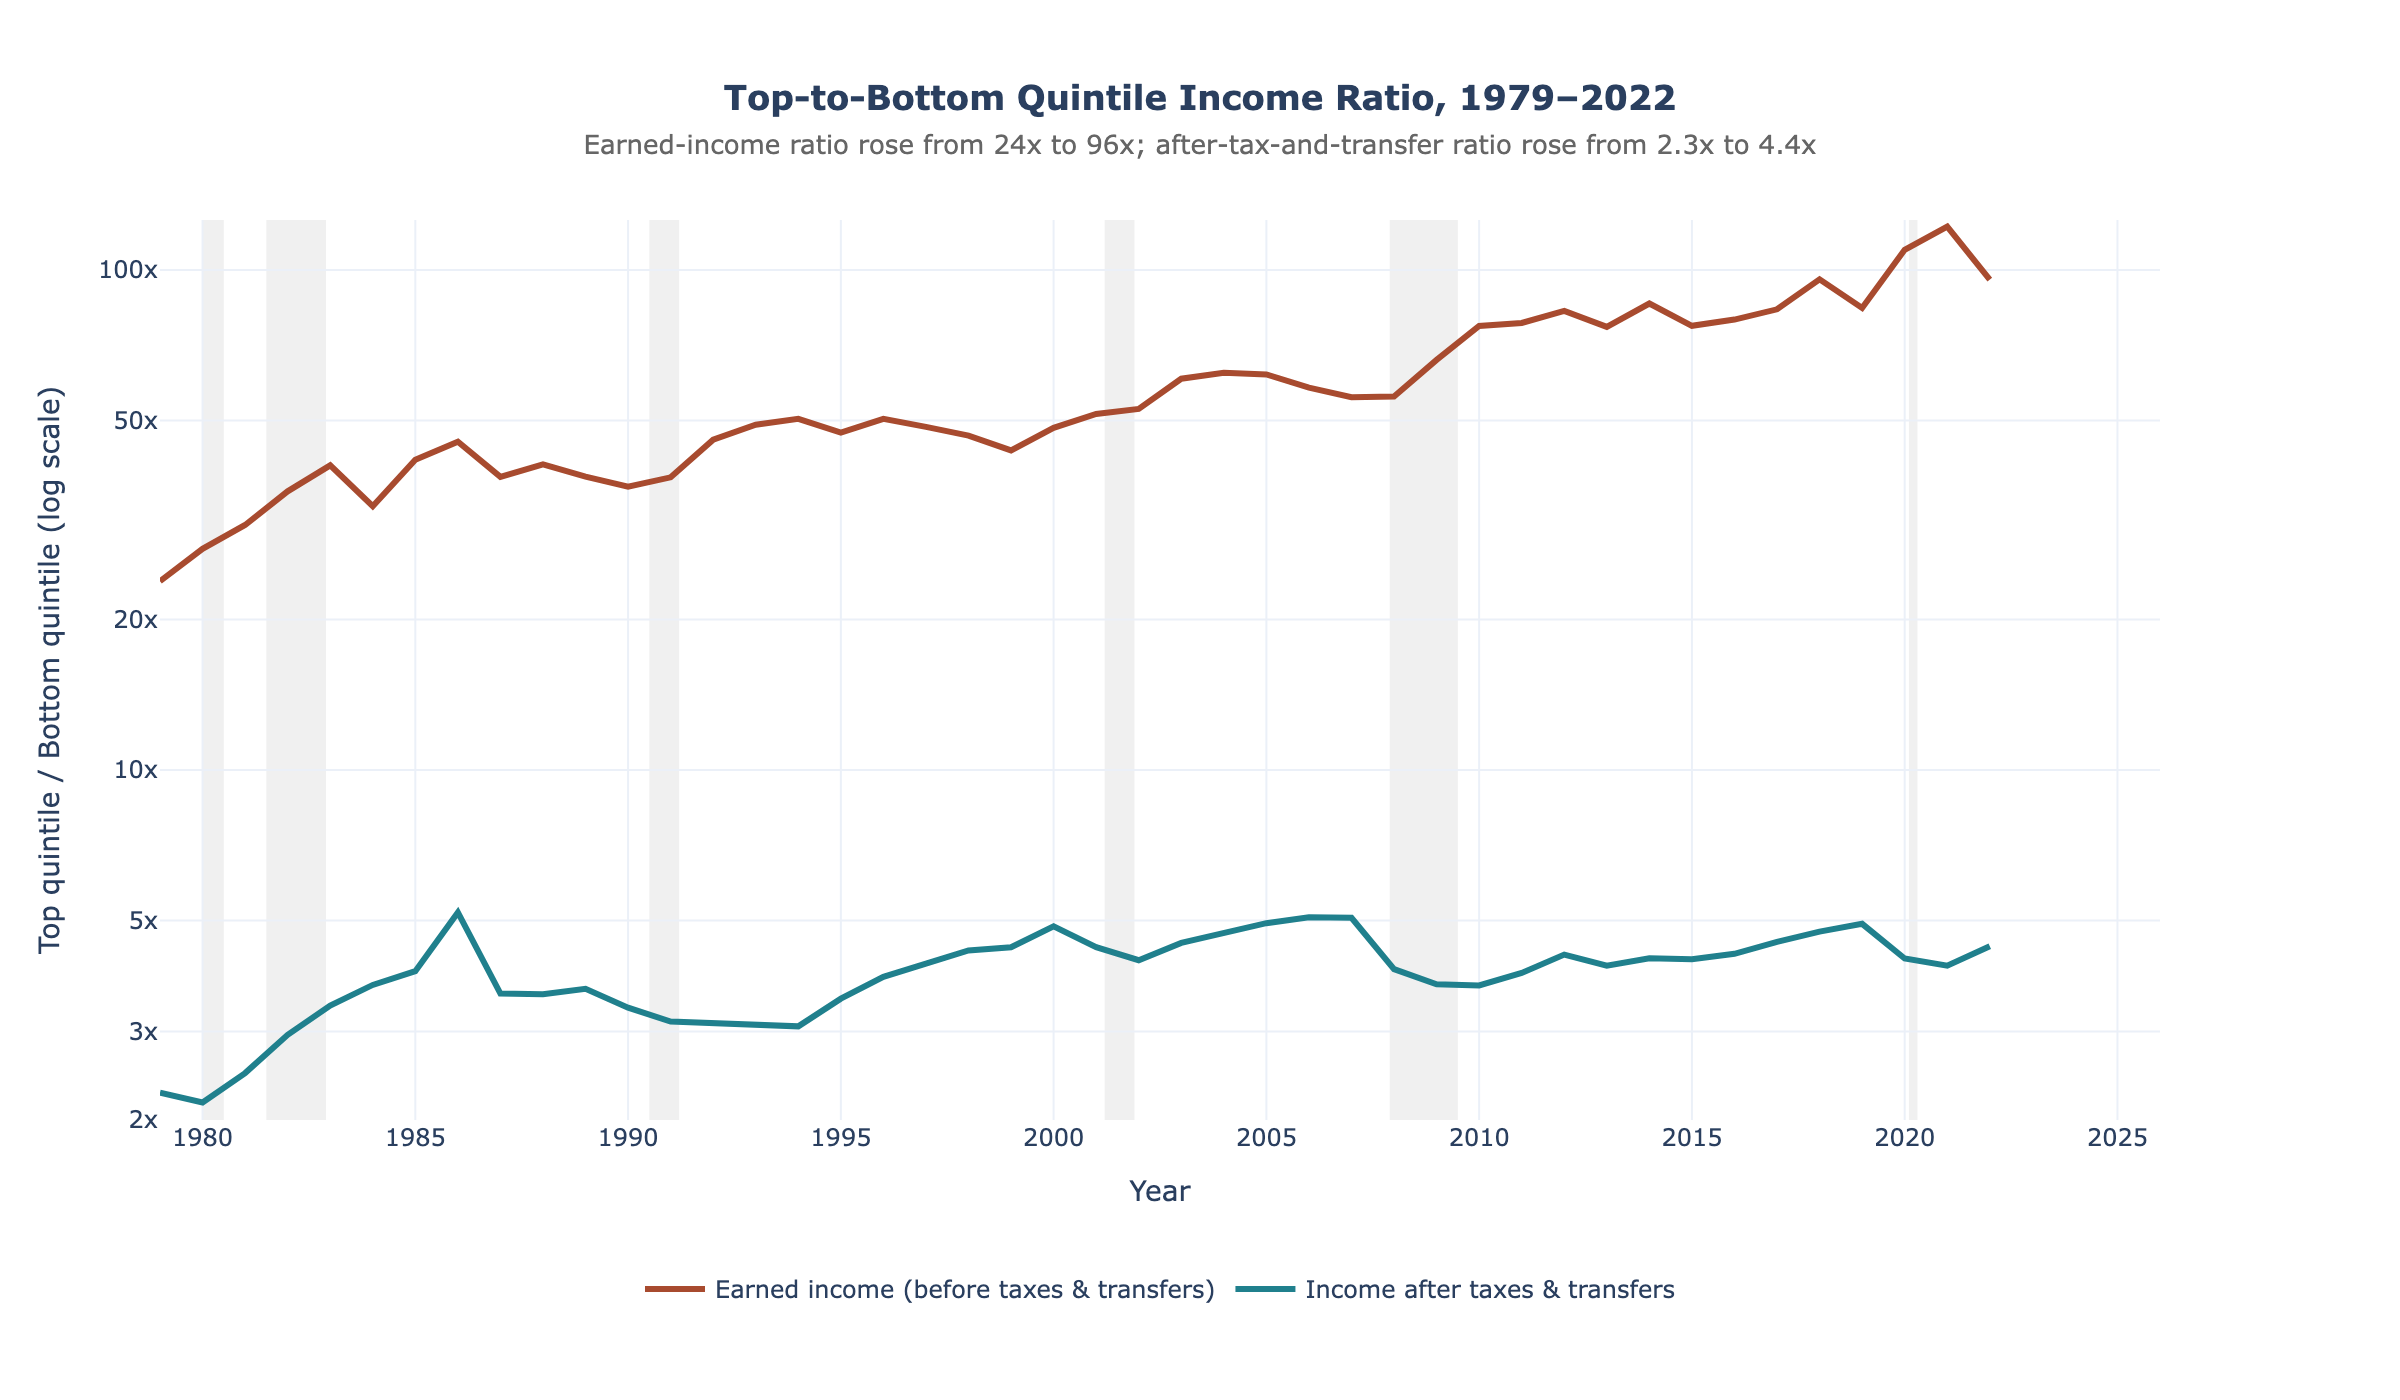
\includegraphics[width=0.95\linewidth]{../output/fig_inequality_ratio_before_after_fisc.png}
\caption{Top-to-bottom quintile income ratio, 1979--2022, comparing earned
income to income after taxes and transfers. Both series are reported on a
common log scale. The vertical gap between the two lines is the
distributional impact of the fiscal system.}
\label{fig:ratio}
\end{figure}

\subsection{The 2022 fiscal cross-section}

Figure~\ref{fig:net} shows the dollar value of taxes paid, government
transfers received, and private transfers received per household per year by
quintile in 2022. The bottom quintile is a net fiscal recipient of about
\$53k per household per year; the second quintile receives about \$26k net;
the middle quintile is roughly neutral (\$1.9k net receipt). The fourth
quintile is a net payer of about \$26k, and the top quintile is a net payer
of about \$125k. These are dollar amounts at the household level, not
percentages of national income.

\begin{figure}[!htb]
\centering
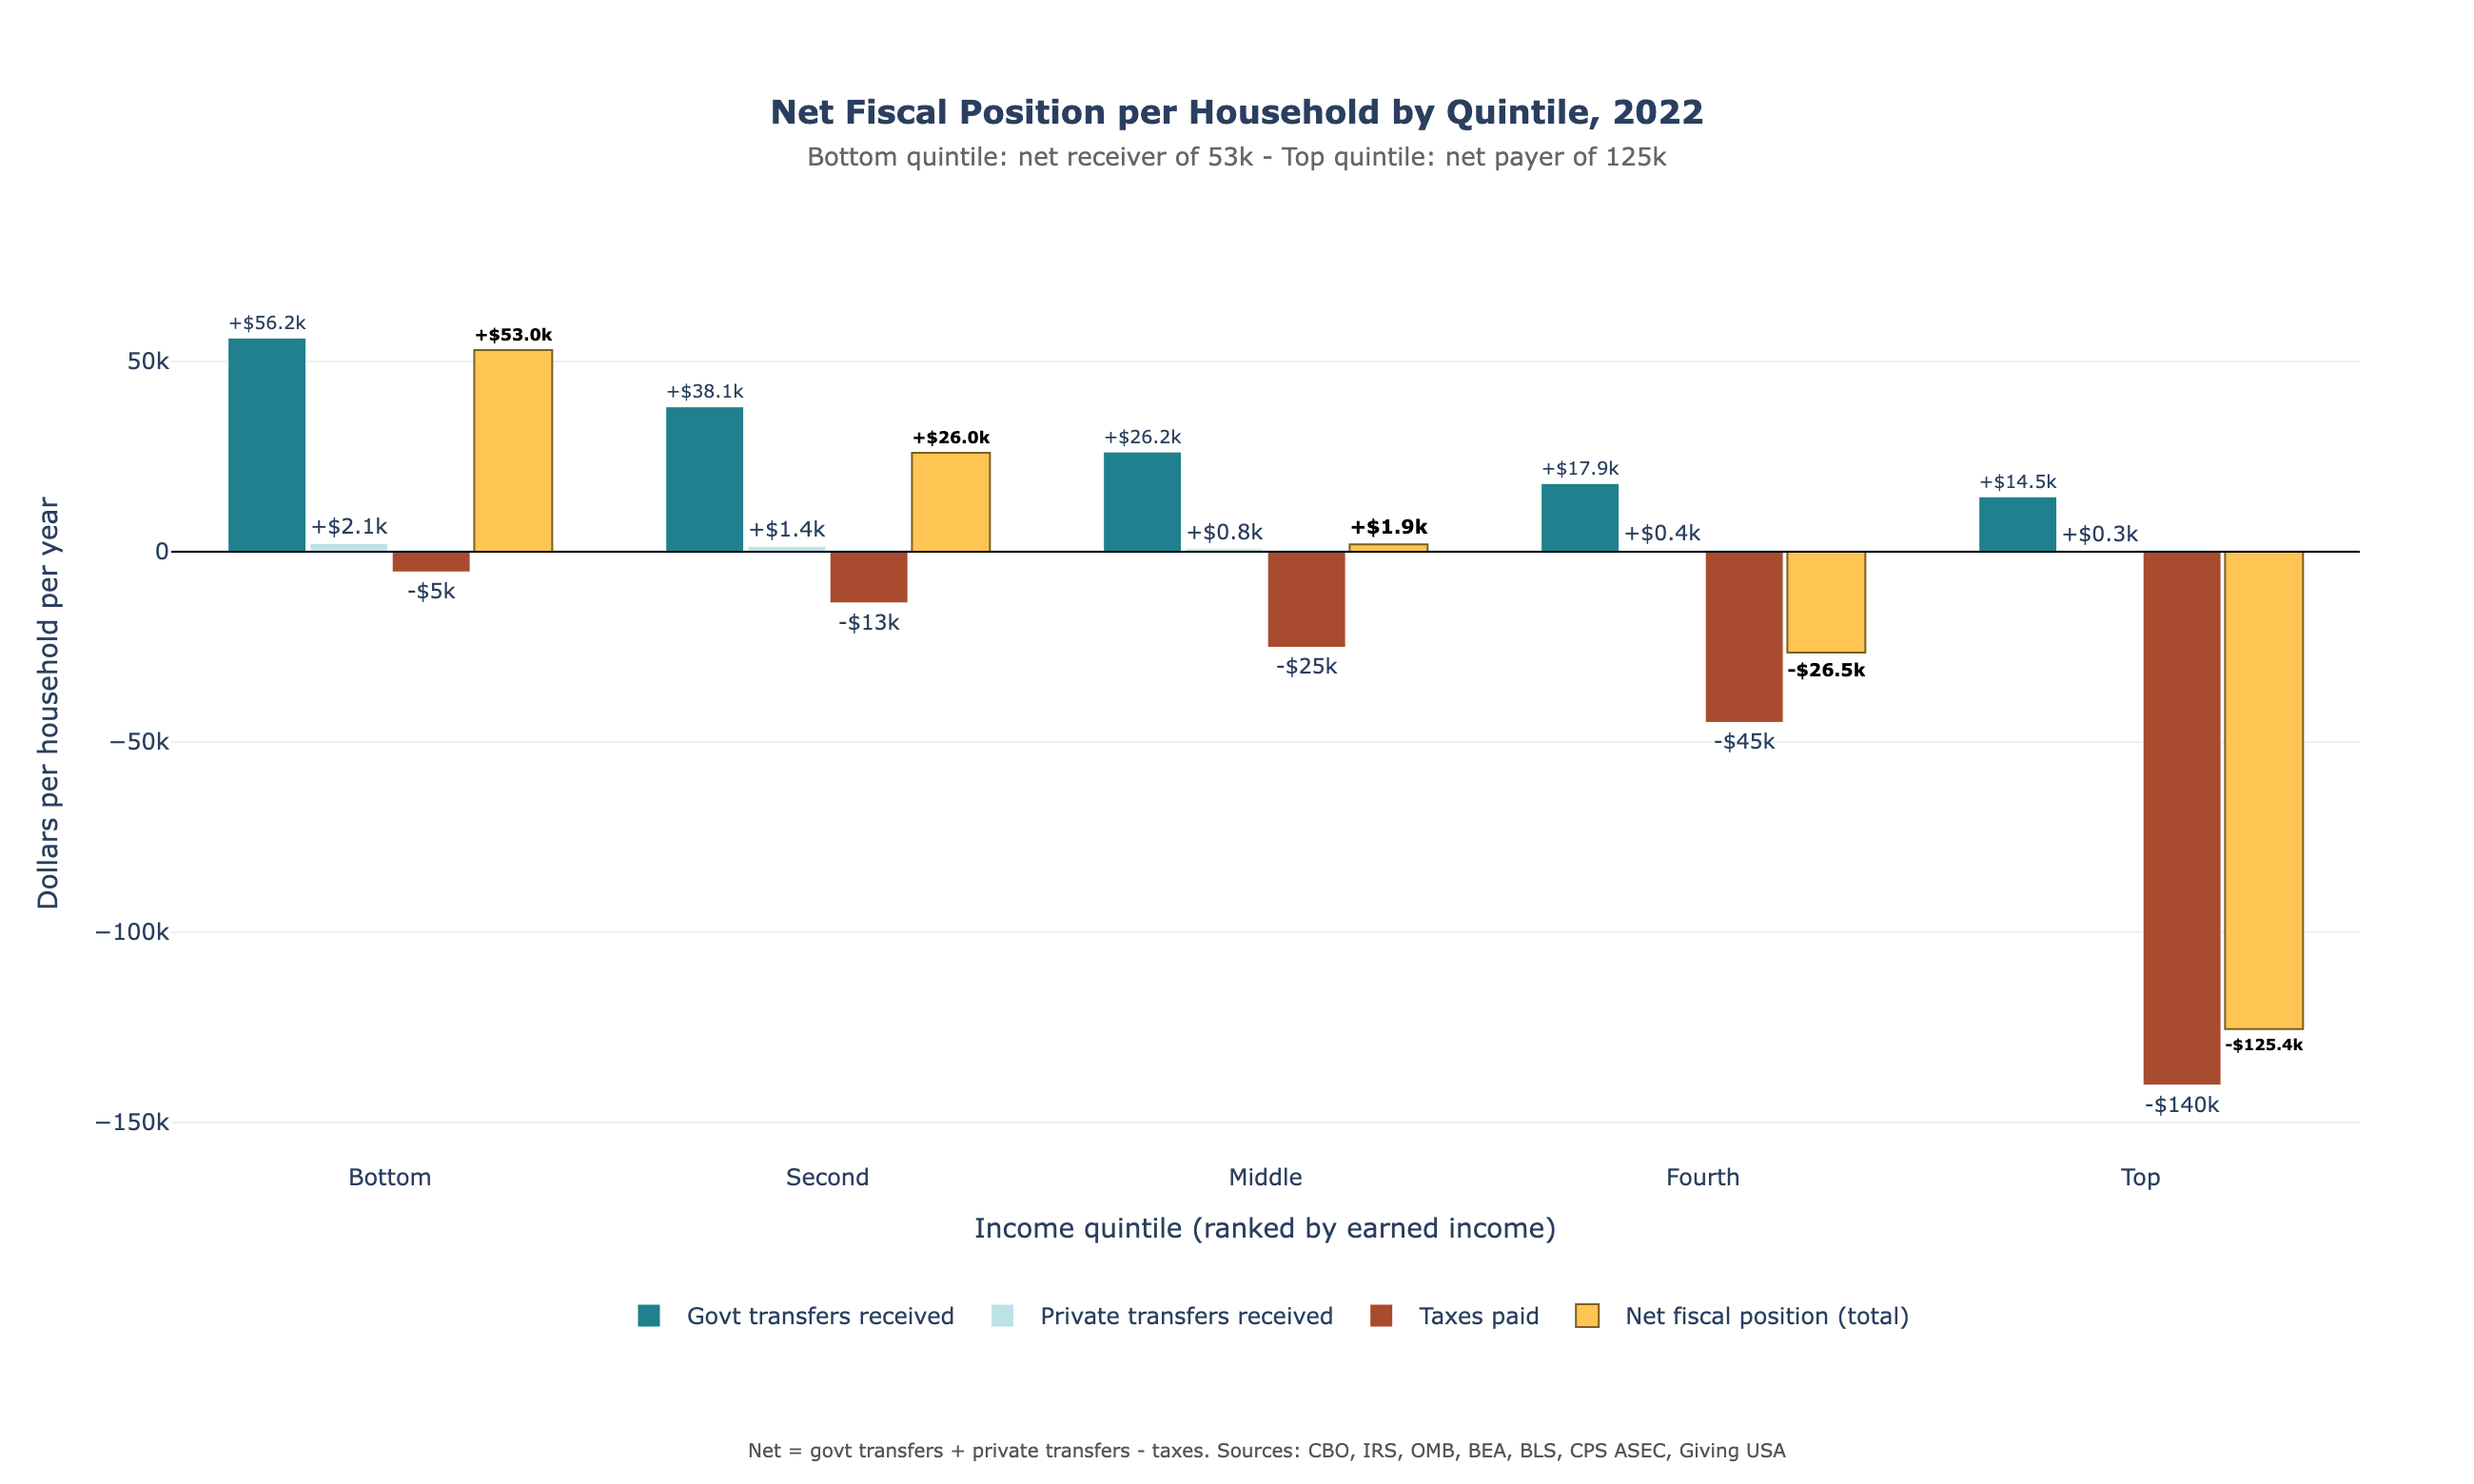
\includegraphics[width=0.95\linewidth]{../output/fig_net_fiscal_position_by_quintile_2022.png}
\caption{Net fiscal position per household by quintile, 2022. The black bars
are the algebraic sum of the other three. Source: panel CSVs in
\texttt{output/}; underlying data from CBO, IRS, OMB, BEA, BLS CEX, CPS ASEC,
and Giving USA.}
\label{fig:net}
\end{figure}

\subsection{Choice of deflator: why True CPI rather than CPI-U}

Any statement about real income growth depends on the price index used to
convert nominal dollars across decades. The default index in most public
discussion --- the Bureau of Labor Statistics' CPI-U --- is known to overstate
the true rate of inflation, and that overstatement compounds over a 43-year
horizon into a meaningful distortion of the headline inequality story. The
panels in this paper are deflated using the Early and Furth (2021) ``True CPI''
alternative index. The reasoning is summarized below; the full derivation lives
in \texttt{src/cpi\_bias\_adjusted\_v3\_dbpi.py} and Figure~\ref{fig:cpi}.

The academic literature has documented three distinct upward biases in the
official CPI-U:

\begin{itemize}[leftmargin=*]
  \item \textbf{Substitution bias} ($\sim$0.5pp/yr). The CPI-U is a
        modified-Laspeyres index that holds expenditure shares roughly
        constant within a basket update cycle. When relative prices change,
        consumers substitute toward cheaper alternatives, but the index does
        not capture this. Estimated at 0.5 percentage points per year by
        Boskin et al. (1996), Lebow and Rudd (2003), and the BLS Chained
        CPI-U project. Removing it produces the second curve in
        Figure~\ref{fig:cpi} (``Chained CPI/PCEPI''), which uses BEA's PCEPI
        for 1979--1999 spliced to BLS's C-CPI-U from 2000 onward.
  \item \textbf{Quality bias.} The CPI assumes a 2022 car, smartphone, or
        television is the same product as its 1979 counterpart, which it
        plainly is not. The Boskin Commission estimated this at
        roughly 0.6pp/yr in the 1990s; Moulton (2018) estimates 0.37pp/yr
        post-2000 reforms; the bias likely fell further to about 0.30pp/yr
        after BLS expanded hedonic adjustment to mobile phones in January
        2018.
  \item \textbf{New-product bias.} Goods that did not exist in the base
        period (smartphones, GPS navigation, video streaming, mRNA vaccines)
        enter the index only after they reach mass adoption, which can be
        years. Their early-period welfare gains never appear in the price
        history.
\end{itemize}

The ``True CPI'' line in Figure~\ref{fig:cpi} compounds the documented
bias schedule on top of the substitution-corrected index, producing a
cumulative inflation estimate of 176\% from 1979 to 2022 --- versus 303\%
for the official CPI-U over the same window. The 127 percentage point gap
is what real-income series in this paper recover relative to series
deflated by CPI-U. The gap is concentrated in components where measurement
difficulties are best documented: the BLS Disease-Based Price Index
(DBPI) for medical care shows roughly 50\% cumulative inflation 1999--2017,
against 75\% for official CPI Medical Care over the same window.

\begin{figure}[!htb]
\centering
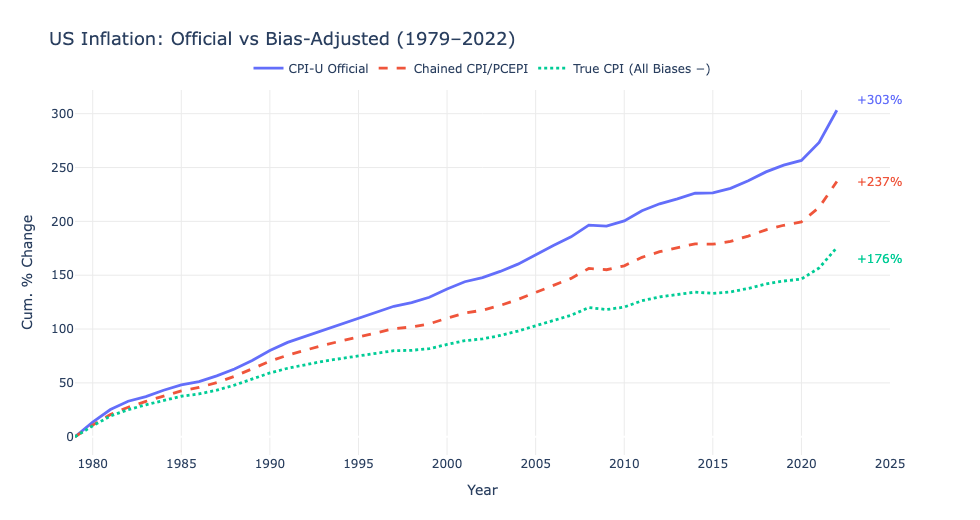
\includegraphics[width=0.95\linewidth]{../output/cpi_headline_v3.png}
\caption{U.S. inflation 1979--2022, three measures. CPI-U is the official
BLS series; Chained CPI splices BEA's PCEPI (1979--1999) to BLS's C-CPI-U
(2000+) and removes substitution bias only; True CPI further deflates the
chained series for the documented quality and new-product biases at
0.30--0.60pp/yr depending on the era. The 127pp gap between CPI-U and True
CPI by 2022 is the amount by which CPI-U-deflated real series understate
long-run real income growth.}
\label{fig:cpi}
\end{figure}

Why this matters for the inequality narrative: deflating with CPI-U makes
real income growth look smaller for everyone, but the effect is not
distributionally neutral. The bottom quintile's real after-tax-and-transfer
income grew by about 129\% over 1979--2022 under True CPI; under CPI-U the
same nominal change produces only about 33\% real growth. The qualitative
story shifts from ``every quintile gained substantially in real terms'' to
``the bottom quintile barely moved'' --- not because the dollar flows
changed, but because of which deflator was used. Choosing a deflator known
to overstate inflation by roughly 0.9pp/yr is therefore not a neutral
modeling choice; it is itself a determinant of the narrative.

This paper uses True CPI throughout for two reasons: (a) it more accurately
reflects the basket of goods households actually consumed each year, given
quality and product-mix changes that the official index misses; and (b) it
is the index used by Gramm, Ekelund, and Early in \emph{The Myth of
American Inequality}, the closest published precedent for this style of
analysis. Sensitivity to deflator choice can be reproduced by re-running
the charts against the \texttt{CPI\_U\_idx} column of
\texttt{cpi\_adjusted\_v3\_dbpi\_1979\_2022.csv}, which is included in the
same output file.

\subsection{Real income growth, 1979--2022}

Figure~\ref{fig:real_iat} reports real income after taxes and transfers by
quintile from 1979 to 2022, deflated using the Early and Furth (2021) ``True
CPI'' alternative price index. After 43 years, the real after-tax-and-transfer
income of the bottom quintile has risen by 129\%, the middle quintile by
201\%, and the top quintile by 349\%. Every quintile has experienced positive
real growth in income that is actually available for consumption.

The contrast with earned income is sharp: real earned income for the bottom
quintile has \emph{fallen} by 48\% over the same period (Figure~\ref{fig:real_earned}),
even as their real after-tax-and-transfer income rose. The fiscal system
absorbs the lost earnings entirely and turns them into a small net gain.

\begin{figure}[!htb]
\centering
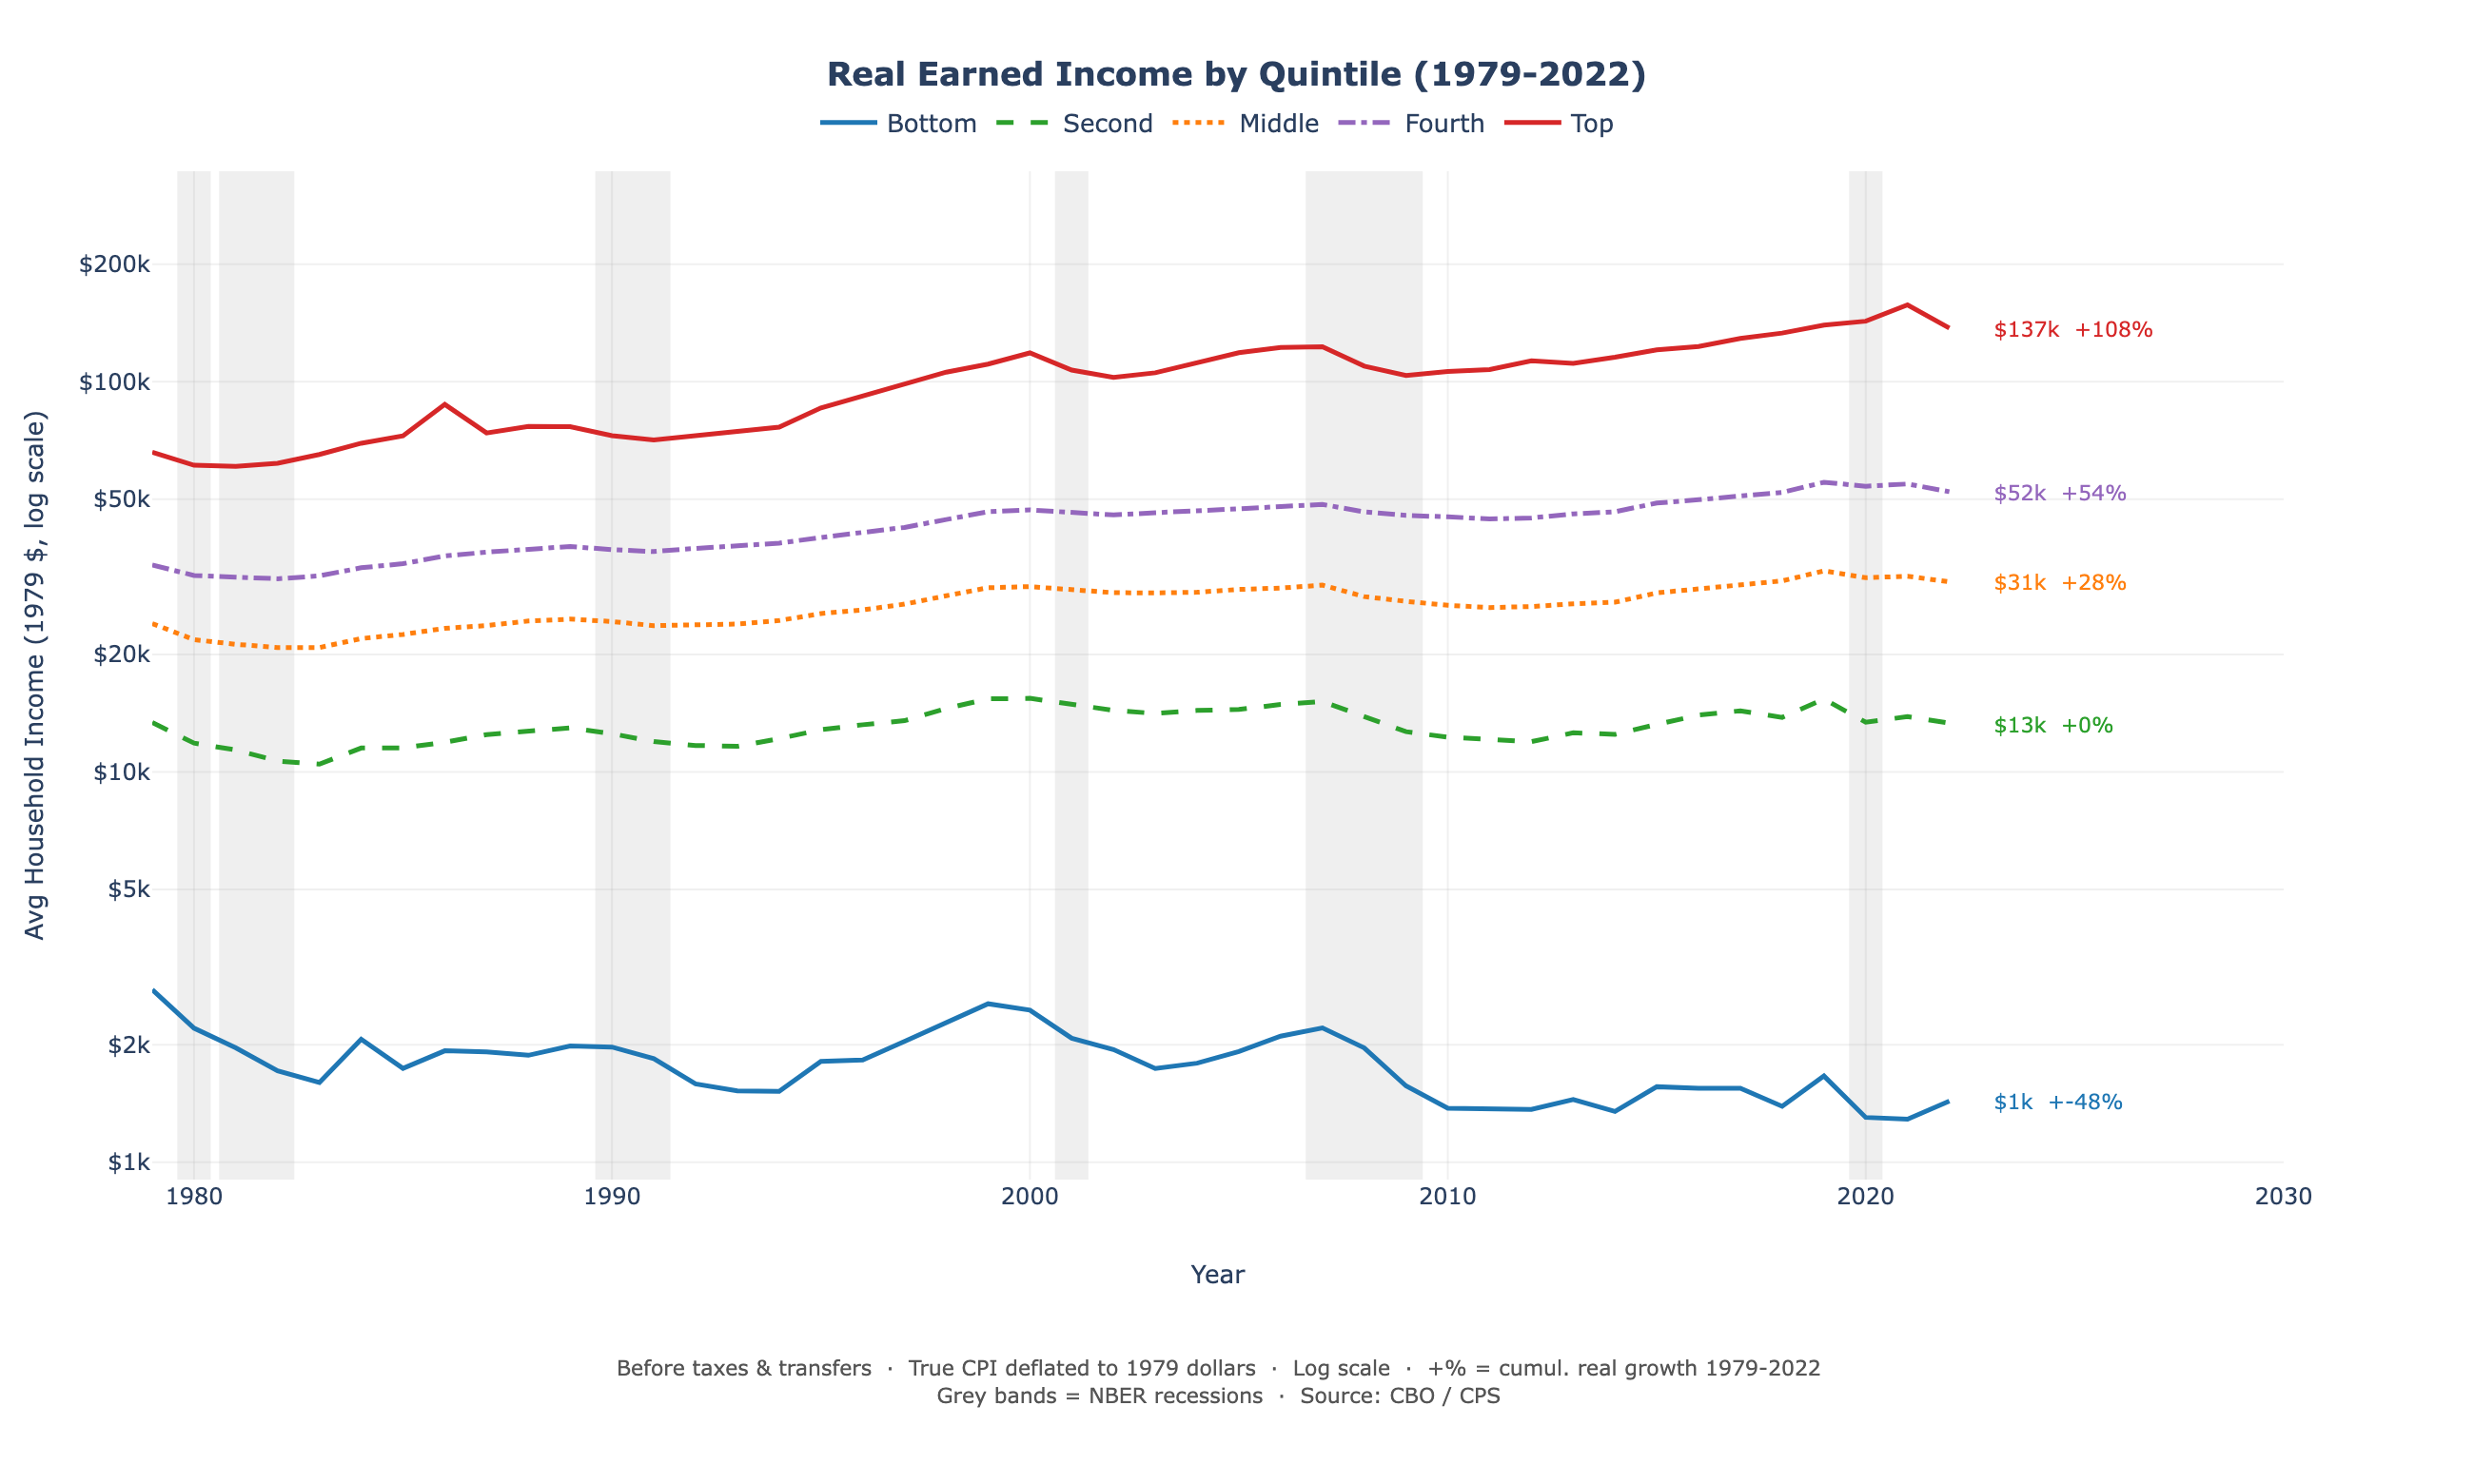
\includegraphics[width=0.95\linewidth]{../output/fig_real_earned_income_by_quintile.png}
\caption{Real earned income by quintile, 1979--2022. Deflated using Early
and Furth (2021) True CPI. Real earned income at the bottom of the
distribution has \emph{fallen} since 1979, while the top has more than
doubled.}
\label{fig:real_earned}
\end{figure}

\begin{figure}[!htb]
\centering
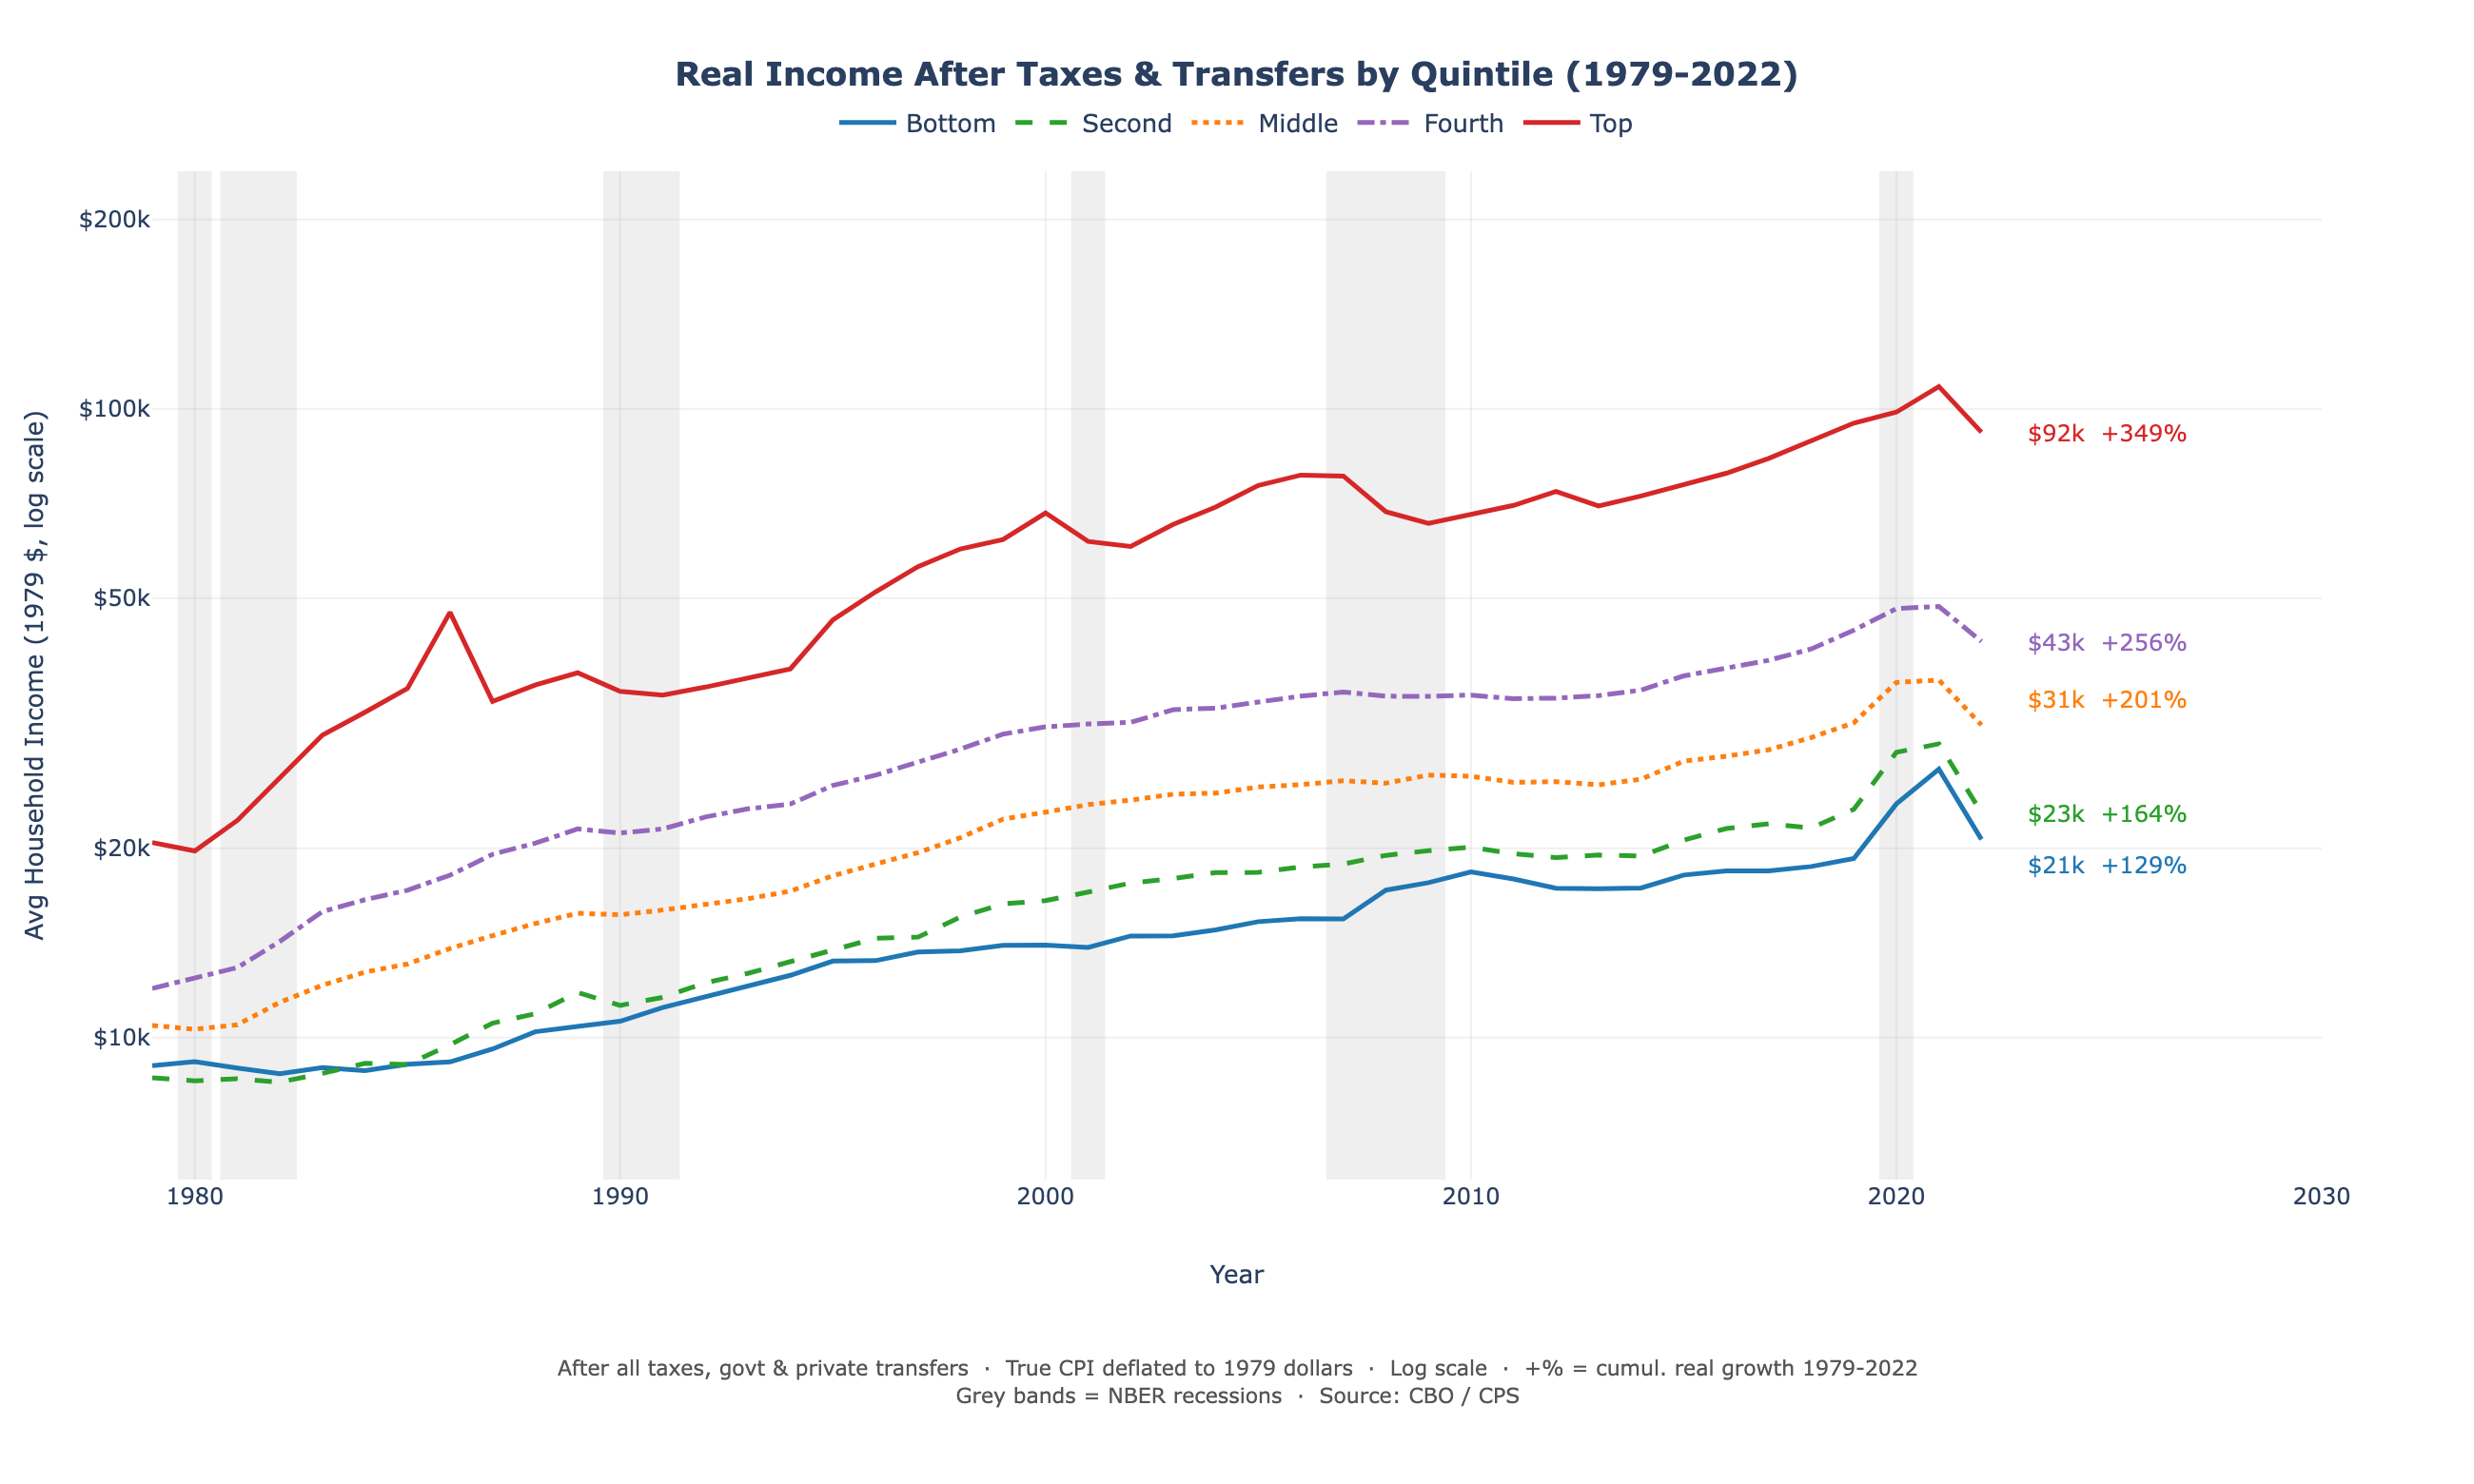
\includegraphics[width=0.95\linewidth]{../output/fig_real_income_after_taxes_transfers_by_quintile.png}
\caption{Real income after taxes and transfers by quintile, 1979--2022. Once
taxes and transfers are accounted for, every quintile has experienced
positive real growth.}
\label{fig:real_iat}
\end{figure}

\subsection{A note on quintile ordering in the early years}

A careful reader will notice that in Figure~\ref{fig:real_iat} the Bottom
and Second quintile lines nearly overlap (and slightly cross) for the first
few years of the panel. This is not a measurement error but a real feature
of the late-1970s post-fisc distribution. In 1979 the per-household IAT
for the bottom quintile is \$9{,}029, slightly above the second quintile's
\$8{,}637. The full numerical ordering violations occur in 1979--1983 and
briefly in 1985.

Two factors drive this. First, the bottom quintile in the late 1970s was
disproportionately retired-elderly households living on Social Security:
their earned income was very low (about \$2{,}800 in 1979), but they
received large OASI benefits (about \$8{,}100 per household) and paid
almost no income tax (retirement income was largely untaxed in that era).
Second, the second quintile was disproportionately working households at
the bottom of the wage distribution: they earned roughly five times more
in the market (\$13{,}400) but paid roughly four times more in taxes
(\$7{,}800), and received only \$3{,}000 in transfers because they were
too young for Social Security and not poor enough for cash welfare.

The ordering normalizes after about 1985 for three reasons: the
Earned Income Tax Credit became more generous (raising second-quintile
post-tax income), AFDC and other cash welfare programs were
tightened (lowering bottom-quintile transfers), and the elderly-retired
share of the bottom quintile gradually fell as more two-earner working
households entered the bottom of the earned-income distribution. Strictly
increasing post-fisc income across quintiles is therefore not a property
the panel imposes; it is something that emerged endogenously over time as
the demographic composition of the bottom quintile shifted.

\subsection{Effective tax rates}

Figure~\ref{fig:eff} plots a signed effective tax rate, \(({T - G - P})/{E}\),
by quintile from 1979 to 2022. The bottom quintile's signed rate has fallen
sharply over time and is now strongly negative (the household receives far
more in transfers than it pays in taxes). The middle quintile's rate has
fallen from roughly 30\% positive in 1979 to roughly zero in 2022. The top
quintile pays approximately 33\% of earned income on net.

\begin{figure}[!htb]
\centering
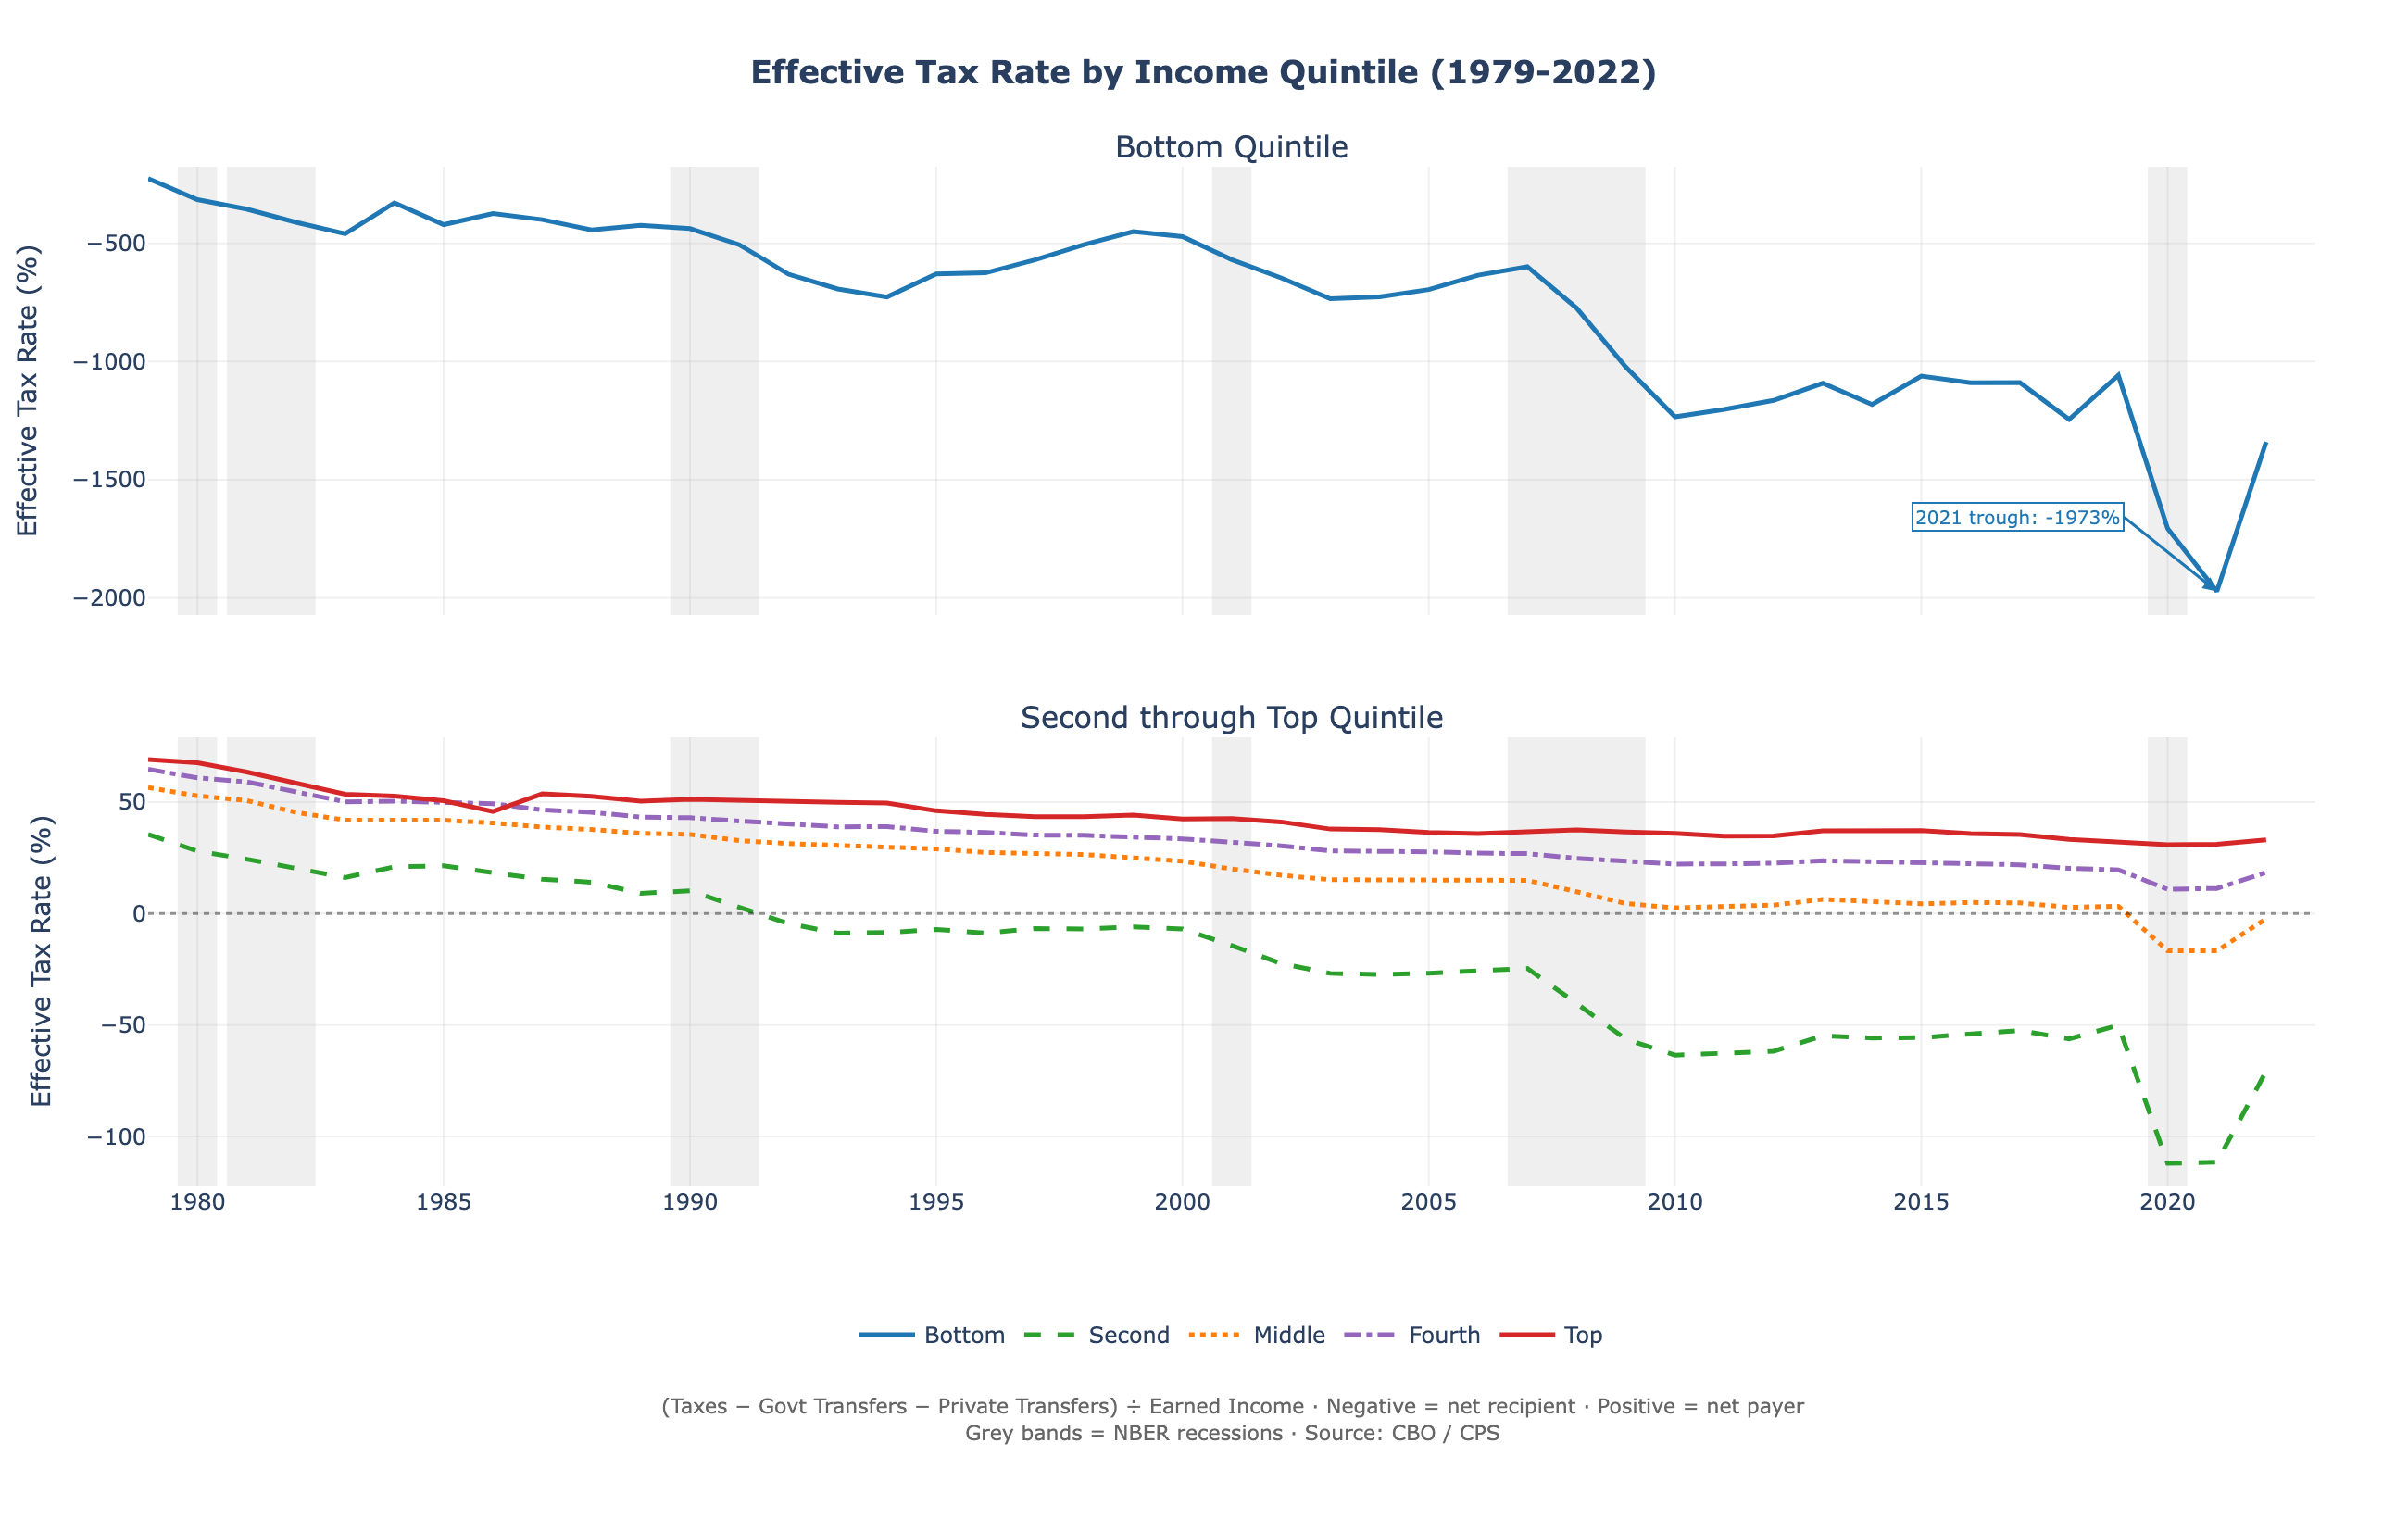
\includegraphics[width=0.95\linewidth]{../output/fig_effective_tax_rate_by_quintile.png}
\caption{Signed effective tax rate by income quintile, 1979--2022. The
numerator is taxes paid minus all transfers received; the denominator is
earned income.}
\label{fig:eff}
\end{figure}

\subsection{The very top of the distribution}

Figure~\ref{fig:top_groups} reports real income after taxes and transfers
for groups above the top quintile: the Top 1\%, Top 0.1\%, Top 0.01\%, Top
0.001\%, and the Forbes 400 (years vary by data availability). The signed
effective tax rate for the Forbes 400 in 2022 is 26.1\%, lower than the Top
1\% rate of 31.6\%. The differential reflects the larger share of capital
gains in AGI at the very top (taxed at preferential rates) and the cap on
payroll taxes.

\begin{figure}[!htb]
\centering
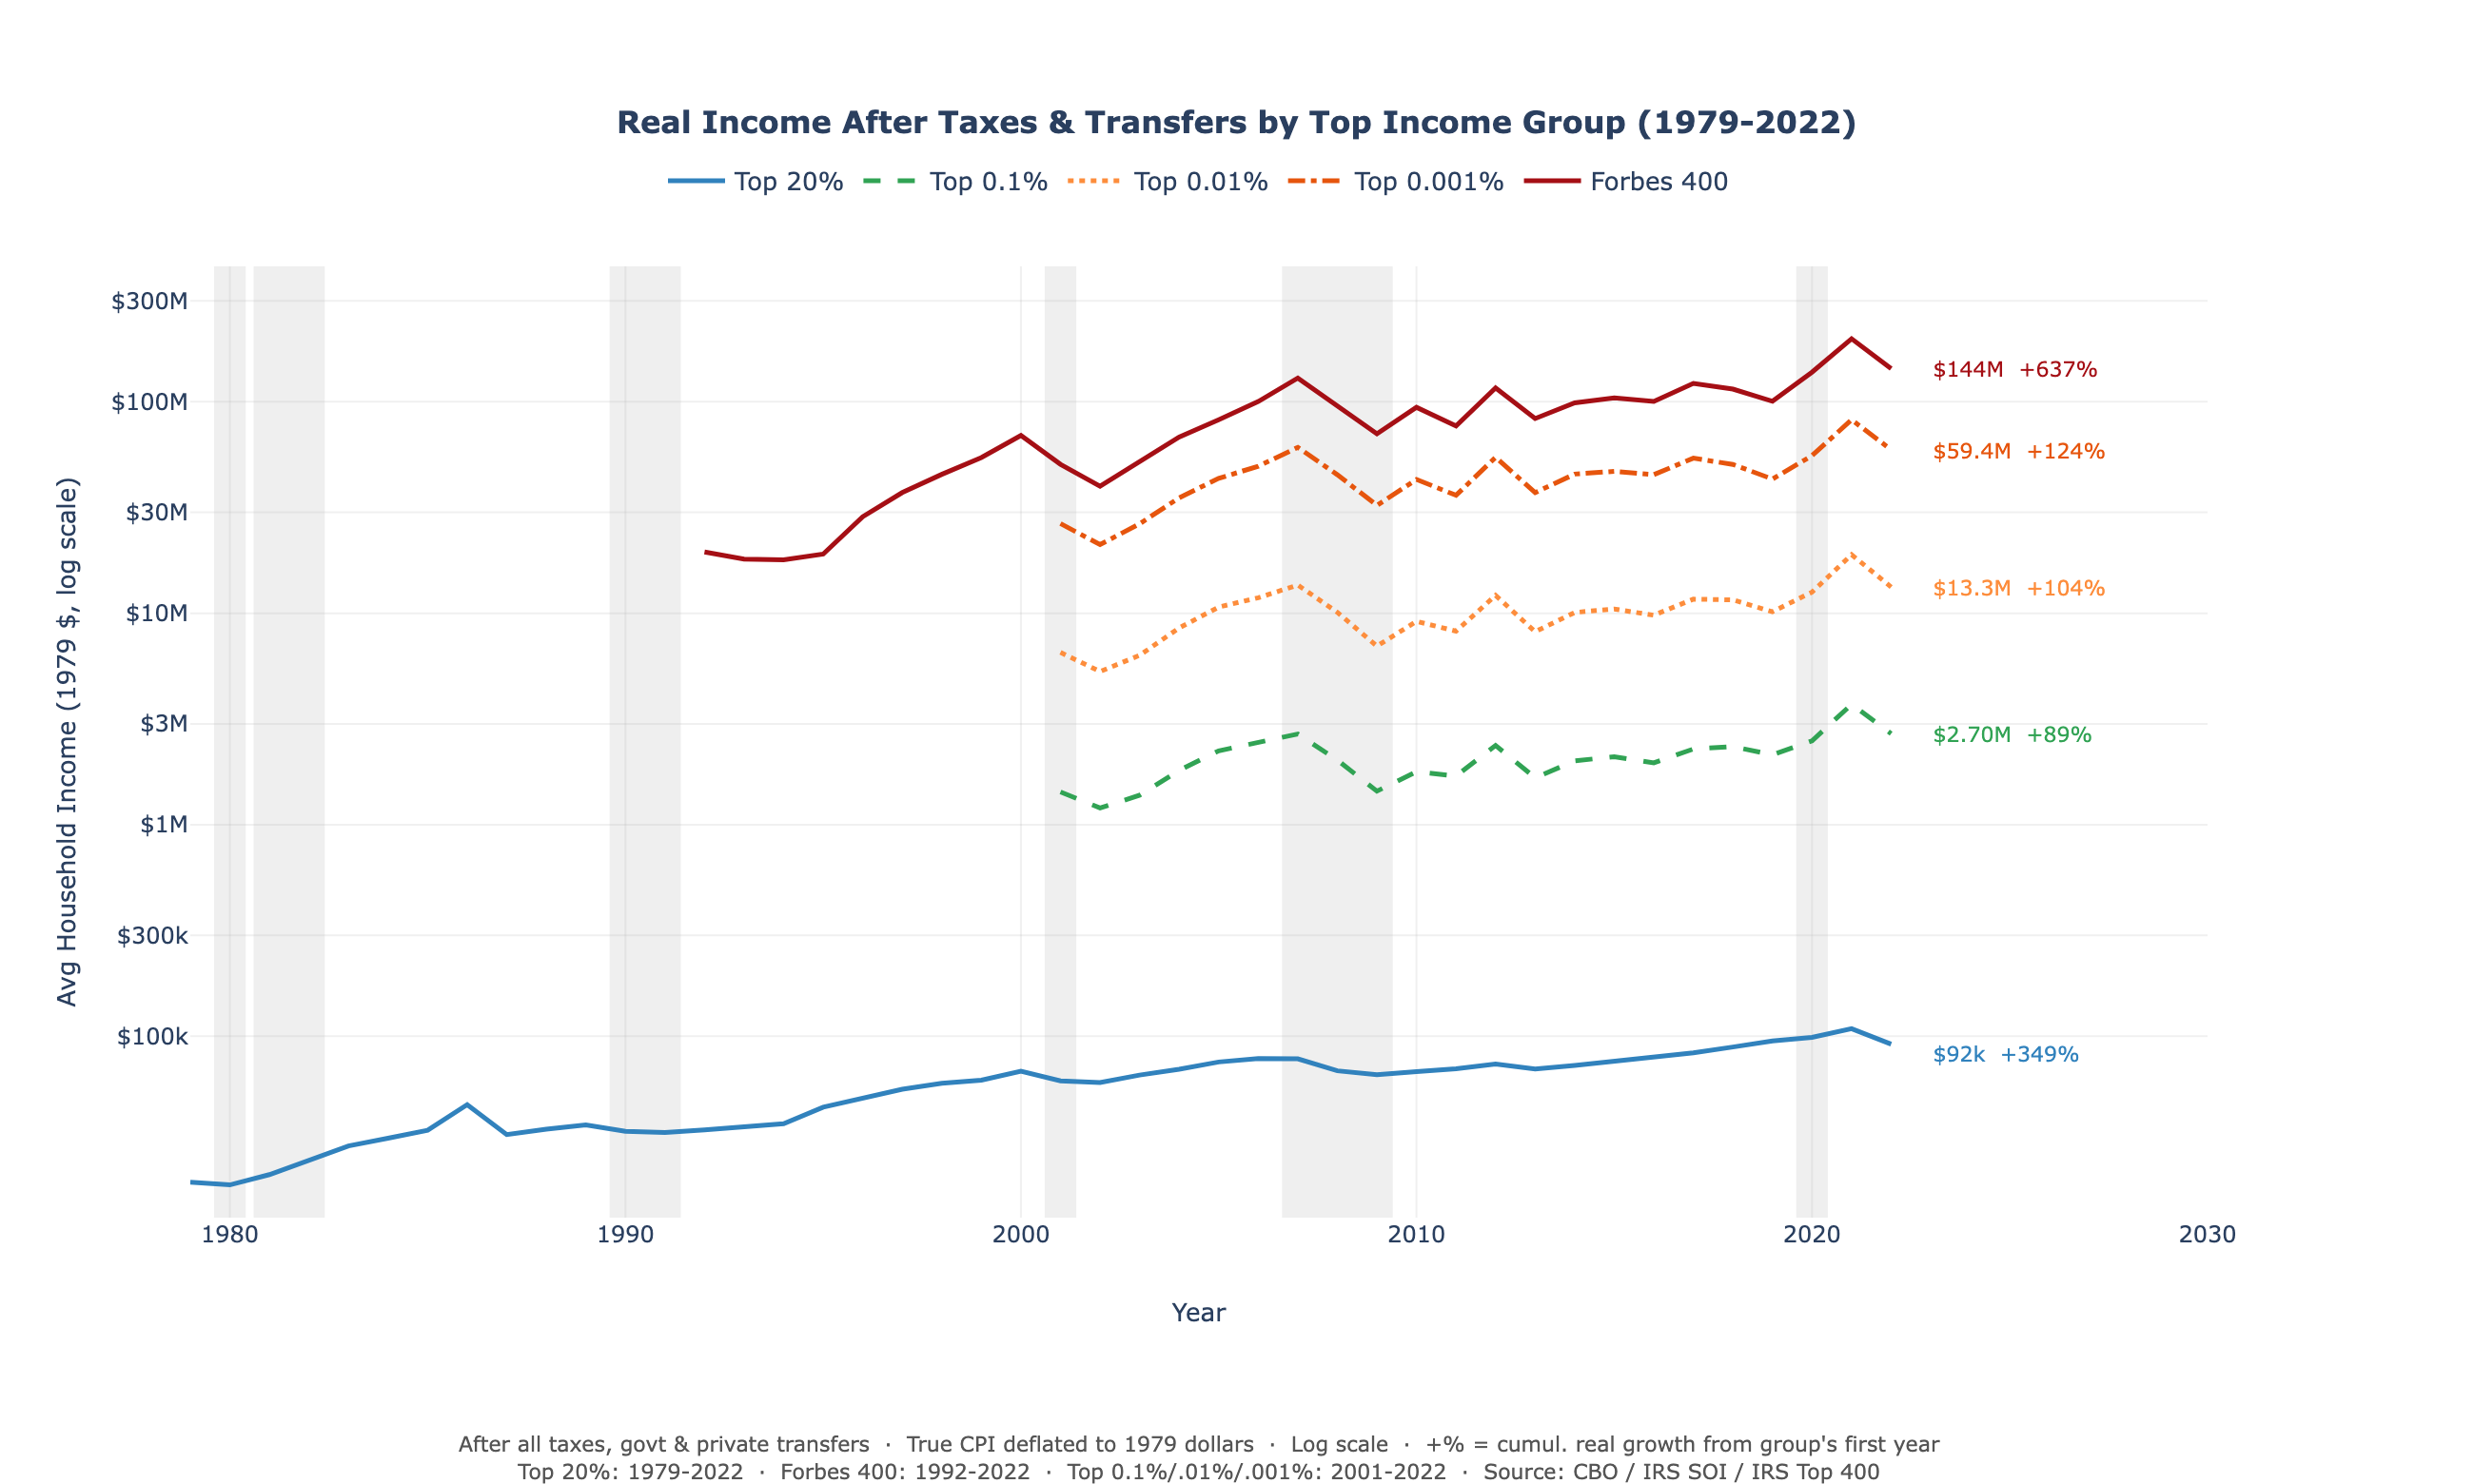
\includegraphics[width=0.95\linewidth]{../output/fig_real_income_after_taxes_transfers_top_groups.png}
\caption{Real income after taxes and transfers for ultra-top groups,
1979--2022 (years vary by data availability).}
\label{fig:top_groups}
\end{figure}

% =============================================================================
\section{Discussion}
% =============================================================================

The size of the discrepancy between the Census ``money income'' measure and
a complete post-fisc measure is large in both cross-section and time series.
In 2022, the bottom quintile receives \$56k of government transfers per
household per year on average, of which a large share is in-kind --- not
counted by the Census construct. The top quintile pays \$140k of taxes per
household per year, none of which is netted out of the Census construct.
The combined effect is to shrink the top-to-bottom quintile gap by an order
of magnitude (96$\times$ becomes 4.4$\times$).

This does not imply that inequality is fictional, nor that distributional
concerns should be set aside: the underlying \emph{earned-income} ratio of
96$\times$ is a real reflection of differences in market productivity. But
it does mean that any claim about the trajectory or level of inequality
needs to specify which income concept is being measured. The choice of
concept is consequential: in 1979 the bottom-quintile household took home
about 22\% more in transfers than it paid in taxes; in 2022 it takes home
about 14$\times$ more.

\subsection{Limitations and open questions}

Several judgment calls are baked into the panel and should be flagged.

\begin{itemize}[leftmargin=*]
  \item \textbf{Medicare valuation.} The panel reports Medicare \emph{net of}
        beneficiary-paid Part B/D premiums and cost-sharing. An alternative
        is to value Medicare at its insurance-equivalent value, which is
        substantially lower than the gross outlay, particularly at the top
        end of the senior distribution.
  \item \textbf{Tax incidence on corporate income.} We exclude corporate
        income tax from the household burden. The tax-incidence literature is
        not unanimous about whether the burden falls primarily on capital or
        on labor; including it shifts both the level and the slope of
        Figure~\ref{fig:eff}.
  \item \textbf{Private transfer methodology.} The Component C approach
        (multiplying each Giving USA category by a fixed household-directed
        fraction) gives an estimate, not a measurement. The fractions for
        Religion (5\%), Health (8\%), and International Affairs (25\%) are
        defensible as central estimates but have wide bounds. Sensitivity
        analysis using upper and lower bounds for those fractions is
        possible from the panel.
  \item \textbf{Census deflator.} We use the Early and Furth (2021) True CPI
        index. The standard CPI-U over-states inflation by roughly 0.5--0.8
        percentage points per year; using the CPI-U instead of the True CPI
        would lower the measured real growth of every quintile.
\end{itemize}

% =============================================================================
\section{Proposed extensions}
% =============================================================================

This work suggests several directions for additional analysis that the
existing panel infrastructure can support without substantial new data
collection.

\subsection{Decomposition of the 1979--2022 IAT change}

A Shapley-style decomposition of the change in real after-tax-and-transfer
income for each quintile, allocating the total to four components: change
in earned income, change in transfers received, change in taxes paid, and
change in the implicit price index. This would clarify how much of each
quintile's gain over four decades is attributable to market earnings versus
the fiscal system.

\subsection{Replication using alternative tax-incidence assumptions}

Re-run the panel under alternative assumptions for who bears the corporate
income tax burden (100\% capital, 50/50 capital--labor, 100\% labor) and
report the resulting effective rates. The Auerbach (2018) and Suarez
Serrato--Zidar (2016) literature suggests this is a meaningful sensitivity.

\subsection{Real consumption analogues}

The companion BLS Consumer Expenditure Survey panel already feeds the S\&L
sales-tax distribution; the same data can be used to construct a household
real-consumption series by quintile, providing a direct test of whether
consumption inequality has tracked income inequality (Krueger and Perri 2006
suggest it has not).

\subsection{Cross-cohort mobility}

The panel as constructed treats each year's quintile membership as
independent. The Panel Study of Income Dynamics (PSID) and IRS Statistics of
Income longitudinal samples allow the same income concepts to be computed
across cohorts, permitting an explicit test of upward and downward mobility
in post-fisc terms over the past four decades.

% =============================================================================
\section{Reproducibility}
% =============================================================================

All seven Python scripts and the underlying CSV outputs are available at
\href{https://github.com/Patrickkp1/tax-transfer-inequality}{github.com/Patrickkp1/tax-transfer-inequality}.
Each script is
self-contained, walks up its own directory tree to find the
\texttt{data/raw/} folder, and can be re-run end-to-end on any UNIX-like
machine with Python 3.10+, pandas, numpy, openpyxl, and plotly. Total
end-to-end runtime against a full CPS extract is approximately 30 minutes.
Each panel CSV is byte-identical across runs given the same inputs.

% =============================================================================
\begin{thebibliography}{99}

\bibitem{gramm2022} Gramm, P., Ekelund, R., \& Early, J. (2022).
\emph{The Myth of American Inequality: How Government Biases Policy Debate.}
Lanham, MD: Rowman \& Littlefield.

\bibitem{cbo2023} Congressional Budget Office (2023).
\emph{The Distribution of Household Income, 1979--2020.} Supplemental data
tables. \url{https://www.cbo.gov/publication/59509}.

\bibitem{meyer2012} Meyer, B.~D., \& Sullivan, J.~X. (2012). ``Identifying
the Disadvantaged: Official Poverty, Consumption Poverty, and the New
Supplemental Poverty Measure.'' \emph{Journal of Economic Perspectives}
26(3): 111--136.

\bibitem{karen2023} Karen, R. (2023). ``The Distribution of Private
Transfers.'' LIS Working Paper Series No.~851.

\bibitem{early2021} Early, D., \& Furth, S. (2021). ``A Better Price
Index.'' Mercatus Center research paper.

\bibitem{krueger2006} Krueger, D., \& Perri, F. (2006). ``Does Income
Inequality Lead to Consumption Inequality? Evidence and Theory.''
\emph{Review of Economic Studies} 73(1): 163--193.

\bibitem{auerbach2018} Auerbach, A.~J. (2018). ``Measuring the Effects of
Corporate Tax Cuts.'' \emph{Journal of Economic Perspectives} 32(4): 97--120.

\bibitem{yagan2023} Yagan, D. (2023). ``What Is the Average Federal Individual
Income Tax Rate on the Wealthiest Americans?'' \emph{Oxford Review of
Economic Policy} 39(3).

\bibitem{givingusa2014} Giving USA Foundation (2014). \emph{Giving USA
2014 Data Tables.} Indianapolis, IN: Indiana University Lilly Family School
of Philanthropy.

\bibitem{ipums} Flood, S., King, M., Rodgers, R., Ruggles, S., Warren,
J.~R., \& Westberry, M. (2024). \emph{Integrated Public Use Microdata
Series, Current Population Survey: Version 12.0} [dataset]. Minneapolis,
MN: IPUMS. \url{https://cps.ipums.org}.

\end{thebibliography}

\end{document}
